\documentclass[tikz]{standalone}
\begin{document}
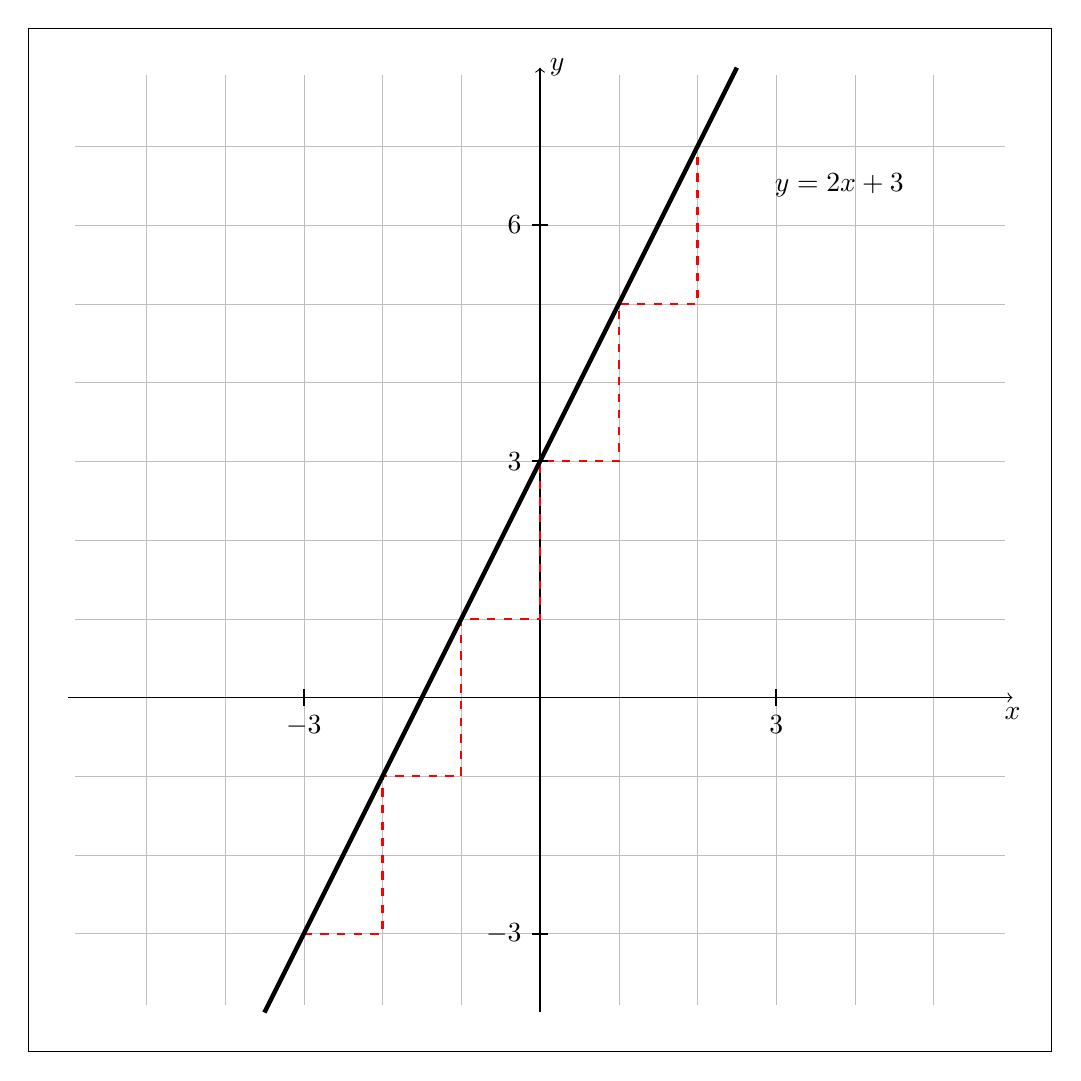
\begin{tikzpicture}[scale=1.0]
\draw[black,fill=white] (-6.5,-4.5) rectangle (6.5,8.5);
%\draw[very thin,color=darkgray,step=3] (-8,-5) grid (8,8.9);
\draw[very thin,color=lightgray,step=1] (-5.9,-3.9) grid (5.9,7.9);
\draw[->] (-6,0) -- (6,0) node[below] {$x$};
\draw[->] (0,-4) -- (0,8) node[right] {$y$};
\node at (3.8, 6.5){$y = 2x+3$};

% draw slope
\draw[dashed,red,thick] (-3,-3) -| ++(1,2) -| ++(1,2) -| ++(1,2) -| ++(1,2) -| ++(1,2);
% draw line and point
\draw[domain=-3.5:2.5,smooth,variable=\x,black,ultra thick] plot ({\x},{2*\x+3});

% tick marks
\foreach \x in {-3,3} 
	\draw [thick] (\x cm,3pt) -- (\x cm,-3pt) node[below] {$\x$};
\foreach \y in {-3,3,6} 
	\draw [thick] (3pt,\y cm) -- (-3pt,\y cm) node[left] {$\y$};
\end{tikzpicture}
\end{document}
